\documentclass{article}

\usepackage[a4paper]{geometry}
\usepackage[ngerman]{babel}
\usepackage[utf8]{inputenc}
\usepackage[T1]{fontenc}
\usepackage{tabularx}
\usepackage{hyperref}
\usepackage{graphicx}
\usepackage{float}

\graphicspath{ {./images/} }

\hypersetup{
    colorlinks=true,
    linkcolor=black,
    filecolor=black,
    urlcolor=black,
}

\begin{document}

\begin{titlepage}
	\begin{flushleft}
		TH Brandenburg \\
		Online Studiengang Medieninformatik \\
		Fachbereich Informatik und Medien \\
		Softwaretechnik \\
		Prof. Dr-Ing. Martin Schafföner
	\end{flushleft}

	\vfill

	\begin{center}
		\Large{Einsendeaufgabe 1: Requirements Engineering}\\[0.5em]
		\large{Sommersemester 2021}\\[0.25em]
		\large{Abgabetermin 27.04.2021}
	\end{center}

	\vfill

	\begin{flushright}
		Maximilian Schulke \\
		Matrikel-Nr. 20215853
	\end{flushright}
\end{titlepage}

\tableofcontents

\newpage

\section{Aufgabenstellung}

Folgende Aufgabenstellung wurde im Moodle-Kurs bekannt gegeben:

\begin{quote}
	Wählen Sie sich ein kleines Entwicklungsprojekt für das gesamte Studienmodul Softwaretechnik und
	verwenden Sie dieses Projekt für alle Lerneinheiten. Beispielsweise ein Tool zur Erfassung von
	Requirements oder ein anderes Tool, das Ihnen im Bereich der Softwaretechnik helfen kann, oder
	ein Tool, welches Sie schon immer mal bauen wollten. Im Verlauf des Moduls können Sie alle Themen
	wie beispielsweise Modellierung oder Testen anhand dieses Projekts praktisch erproben.

	Ermitteln und dokumentieren Sie die Requirements für ihr Projekt!

	\begin{itemize}
		\item Formulieren Sie die Anforderungen als User Stories in der Sprache des Benutzers!
		\item Formulieren Sie Abnahmeszenarien!
		\item Reichern Sie weitere Informationen an, um die Qualitätskriterien für gute Anforderungen zu erfüllen!
	\end{itemize}

	Stellen Sie weiterhin dar, wie, d.h. mit welchen Werkzeugen bzw. in welcher Struktur, Sie diese Requirements verwalten!

	Die Abgabe erfolgt in Form genau einer PDF-Datei. Falls sie Werkzeuge einsetzen, die keinen PDF-Export erlauben, fertigen Sie Screenshots an, die Sie mit der übrigen Beschreibung in eine PDF-Datei einfügen.

	Anmerkungen:
	\begin{itemize}
		\item Der zeitliche Umfang dieser Einsendeaufgabe wird mit durchschnittlich 4 Stunden abgeschätzt
		\item Eine Nachbearbeitung der abgegeben Lösung nach der Deadline ist nicht vorgesehen. Falls Sie Fragen zur Aufgabenstellung haben, fragen Sie diese also bitte im Vorfeld!
	\end{itemize}
\end{quote}

\section{Projekt}

Als Projekt für dieses Semester verwende ich eine Idee, die mir schon seit längerem im Kopf rumgeistert
– einen kleinen, minimalistischen \emph{Tiling Window Manager} für Linux bzw. X11, der deutlich flexibler
und entwicklerfreundlicher ist als bestehende, vergleichbare Software.

\subsection{Zusammenfassung der Domain}

Für den Fall, dass Sie noch keinen Kontakt mit dieser Domain hatten, gehe ich im folgenden kurz darauf ein,
welche Aufgaben ein \emph{Tiling Window Manager} (kurz. \emph{TWM} oder nur \emph{WM}) typischer Weise
übernimmt. Die generelle Aufgabe eines WM's besteht hauptsächlich darin sich um die Kommunikation mit dem
\emph{Window-Server} (i.d.R. X11 oder Wayland auf Linux, Quartz Compositor auf MacOS) zu kümmern, und die
tatsächliche Anordnung der Fenster auf dem Bildschirm zu regeln (in Ebenen, Kacheln etc. – die Möglichkeiten
sind nahe zu unbegrenzt). Typische \emph{Window Manager} von z.B. MacOS können diverse, für uns als Endnutzer
mittlerweile als üblich angesehene, Anordnungen wie Floating, Split-Screen und Fullscreen realisieren. \par
Ein \emph{Tiling Window Managers} hat nun die Besonderheit, dass er anders als von Windows, MacOS oder diversen
Linux Desktop-Umgebungen bekannt, die Aufteilung der Fenster automatisch und bestmöglich regelt. Typischerweise
hat ein \emph{TWM} eine feste Konfiguration mit Layouts, in die er die Fenster einsortieren kann (z.B. ``Master
and Stack``). Somit muss sich der Anwender eines solchen \emph{TWM's} (zumindest initial) nicht selber um die
Anordnung seiner Fenster kümmern. Desweiteren zählt die Möglichkeit, Keybindings zur Navigation oder Veränderung
der Aufteilung zu definieren, zu den typischen Features eines \emph{Tiling Window Managers}.

\subsection{Projekt-Ziel}

Das Problem von bestehenden \emph{Window Managern} ist in der Regel deren Alter (bspw. ist das Projekt ``Toms
Window Manager`` im Jahr 1987 entstanden). Aufgrund des Alters sind viele dieser \emph{Window Manager} noch in
C, C++ oder einer vergleichbaren Sprache verfasst worden und mit der Zeit immer weiter gewachsen. Dies macht es
deutlich schwerer als es sein müsste, grundlegende Änderungen, die nicht von den Entwicklern vorhergesehen waren,
vorzunehmen. \par
Ziel ist es einen \emph{minimalen Window Manager} zu entwickeln, der \emph{durch eigenen Programm-Code konfiguriert}
und erweitert werden kann. Dieses Konzept ist schon öfter Implementiert worden (als Inspiration für dieses Modell
dienen die Projekte \emph{XMonad\footnotemark} und \emph{DWM\footnotemark}), allerdings sind diese Projekte leider
meistens schlecht dokumentiert und haben i.d.R. unnötig komplexe \emph{API's}. Zu den typischen Anwendern dieser
\emph{Window Manager} gehören Entwickler und Power User.

\footnotetext[1]{wurde 2007 erstmals veröffentlicht. Wurde in Haskell geschrieben und wird auch damit
	konfiguriert. Siehe \url{https://xmonad.org/} für weitere Informationen.}
\footnotetext[2]{ist ein äußerst kleiner (unter 2000 Zeilen Source-Code) Window Manager geschrieben in C. Er
	hat keine Konfigurationsdatei und wird durch Patchen des Codes konfiguriert. Siehe \url{https://dwm.suckless.org/}
	für weitere Informationen.}

\section{Erfassung der Anforderungen}

Zur Erfassung der Anforderungen verwende ich das Projektmanagement Feature von GitHub. Dieses hat zumindest im
kleinen Rahmen diverse Vorteile gegenüber herkömmlicher Software für Agile Projekte (z.B. Jira von Atlassian).
Unter anderem Folgende:

\begin{itemize}
	\item Übersichtlicher durch kleineren Umfang und somit leichter zu Bedienen
	\item Direkte Integration mit dem Entwicklungsprozess (Issues können z.B.
	      geschlossen werden sobald ein Feature gemerged wurde)
	\item Nutzer der Software können direkt Issues anlegen
\end{itemize}

Diese Entscheidung hat keine Endgültigkeit. Wenn es ein echtes Team mit einem klaren Vorgehensmodell gibt, können
andere Tools besser geeignet sein. Außerdem sei erwähnt, dass Jira mit diversen Integrationen erweitert werden
kann, um die oben beschriebene Funktionalität nachzurüsten. Zur geordneten Erfassung von Anforderungen, deren
Priorisierung, Kategorisierung und Abnahme, reicht \emph{GitHub Projects} allerdings vorerst vollkommen aus. Es
gibt die Möglichkeit Sprint oder Kanban Boards anzulegen, diese zu automatisieren oder komplett eigene Prozesse
zu integrieren.

\vspace{0.5em}

\begin{figure}[ht]
	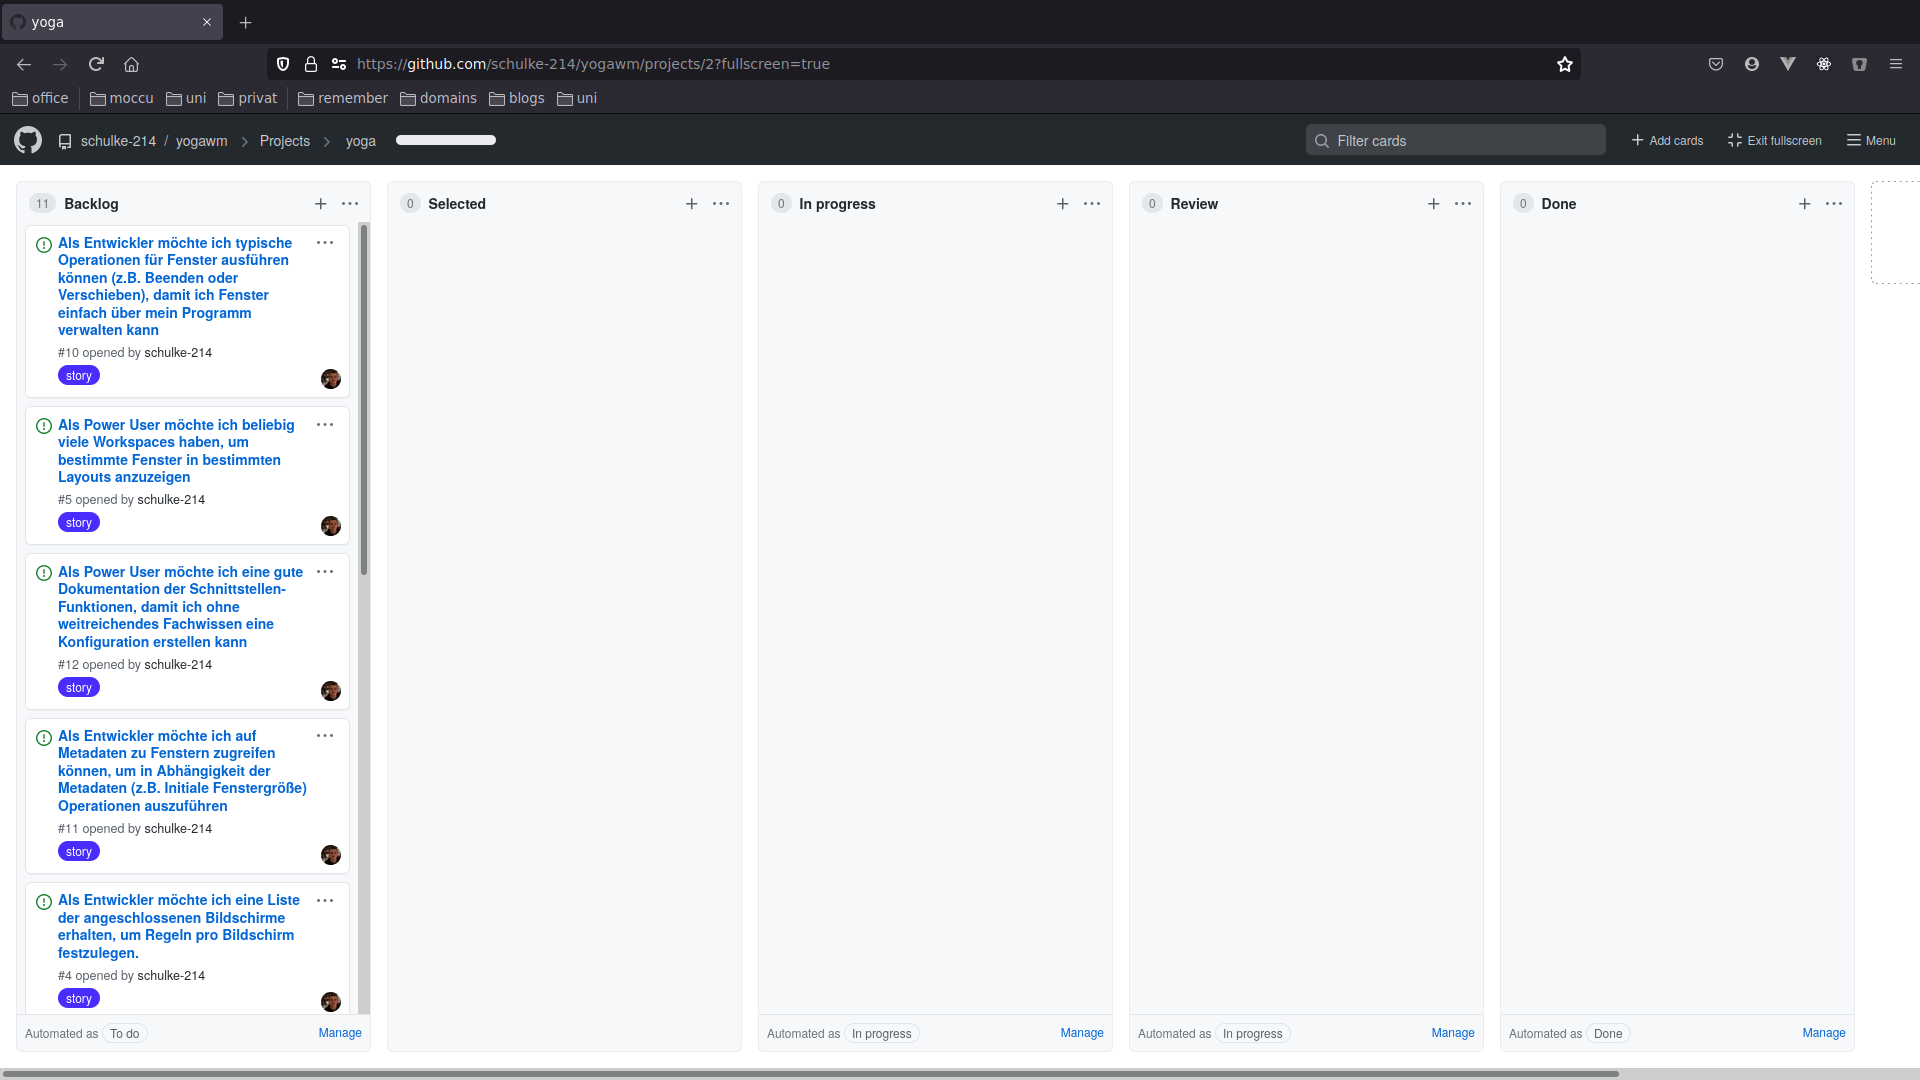
\includegraphics[width=1\textwidth]{github-projects}
	\centering
	\caption{\emph{GitHub Projects} Board}
\end{figure}

\vspace{0em}
\newpage

\section{Anforderungen}

Um die Lesbarkeit zu gewährleisten, habe ich hier eine Kopie des Backlogs aus GitHub Projects eingefügt.
Einen Screenshot des Interfaces finden Sie weiter unten (Abbildung \ref{fig:backlog} auf Seite \pageref{fig:backlog}).

\vspace{1em}

\begin{tabularx}{\textwidth}{|c|X|}
	\hline
	\textbf{ID} & \textbf{Story}                                                                                                                                                                  \\
	\hline
	\#10        & Als Konfigurierender möchte ich typische Operationen für Fenster ausführen können (z.B. Beenden oder Verschieben), damit ich Fenster einfach über mein Programm verwalten kann. \\
	\hline
	\#18        & Als Konfigurierender möchte ich Keyboard-Shortcuts definieren, um meine Maus so selten wie möglich zu verwenden.                                                                \\
	\hline
	\#7         & Als Konfigurierender möchte ich Layouts definieren, damit meine Fenster bestmöglich angeordnet werden.                                                                          \\
	\hline
	\#20        & Als Konfigurierender möchte ich zwischen verschiedenen Workspaces hin und her wechseln, um mehrere Workspaces auf einem Monitor haben zu können.                                \\
	\hline
	\#16        & Als Konfigurierender möchte ich ein Fenster in Fullscreen anzeigen können, damit ich ablenkungsfrei arbeiten kann.                                                              \\
	\hline
	\#19        & Als Konfigurierender möchte ich Fenster zwischen verschiedenen Workspaces verschieben, um die Kontrolle über die angezeigten Fenster je Workspace zu haben.                     \\
	\hline
	\#17        & Als Konfigurierender möchte ich Border für Fenster festlegen können, um zu sehen welches Fenster aktiv ist.                                                                     \\
	\hline
	\#9         & Als Konfigurierender möchte ich eine Statusleiste einbinden können, um den Status, wie z.B. den momentanen Workspace, angezeigt zu kriegen.                                     \\
	\hline
	\#6         & Als Konfigurierender möchte ich Regeln definieren, um Fenster einer Anwendung in einen Workspace einzusortieren.                                                                \\
\end{tabularx}

\begin{tabularx}{\textwidth}{|c|X|}
	\#8  & Als Konfigurierender möchte austauschbare Layouts, um eigene Layouts implementieren und verwenden zu können.                                                        \\
	\hline
	\#12 & Als Konfigurierender möchte ich eine gute Dokumentation der Schnittstellen-Funktionen, damit ich ohne weitreichendes Fachwissen eine Konfiguration erstellen kann.  \\
	\hline
	\#11 & Als Konfigurierender möchte ich auf Metadaten von Fenstern zugreifen können, um in Abhängigkeit der Metadaten (z.B. Initiale Fenstergröße) Operationen auszuführen. \\
	\hline
	\#4  & Als Konfigurierender möchte ich eine Liste der angeschlossenen Bildschirme erhalten, um Regeln pro Bildschirm festzulegen.                                          \\
	\hline
	\#13 & Als Konfigurierender möchte ich einfach Zugriff auf Community Erweiterungen haben, um so wenig wie möglich zu programmieren.                                        \\
	\hline
	\#5  & Als Konfigurierender möchte ich beliebig viele Workspaces haben, um bestimmte Fenster in bestimmten Layouts anzuzeigen.                                             \\
	\hline
	\#15 & Als Konfigurierender möchte ich einfach mit Maus-Events arbeiten, um die Maus als Alternative zur Tastatur verwenden.                                               \\
	\hline
	\#14 & Als Konfigurierender möchte ich Hooks haben, damit ich die Funktionsweise grundlegend beeinflussen kann ohne die Schnittstelle zu Patchen.                          \\
	\hline
\end{tabularx}

\begin{figure}[ht]
	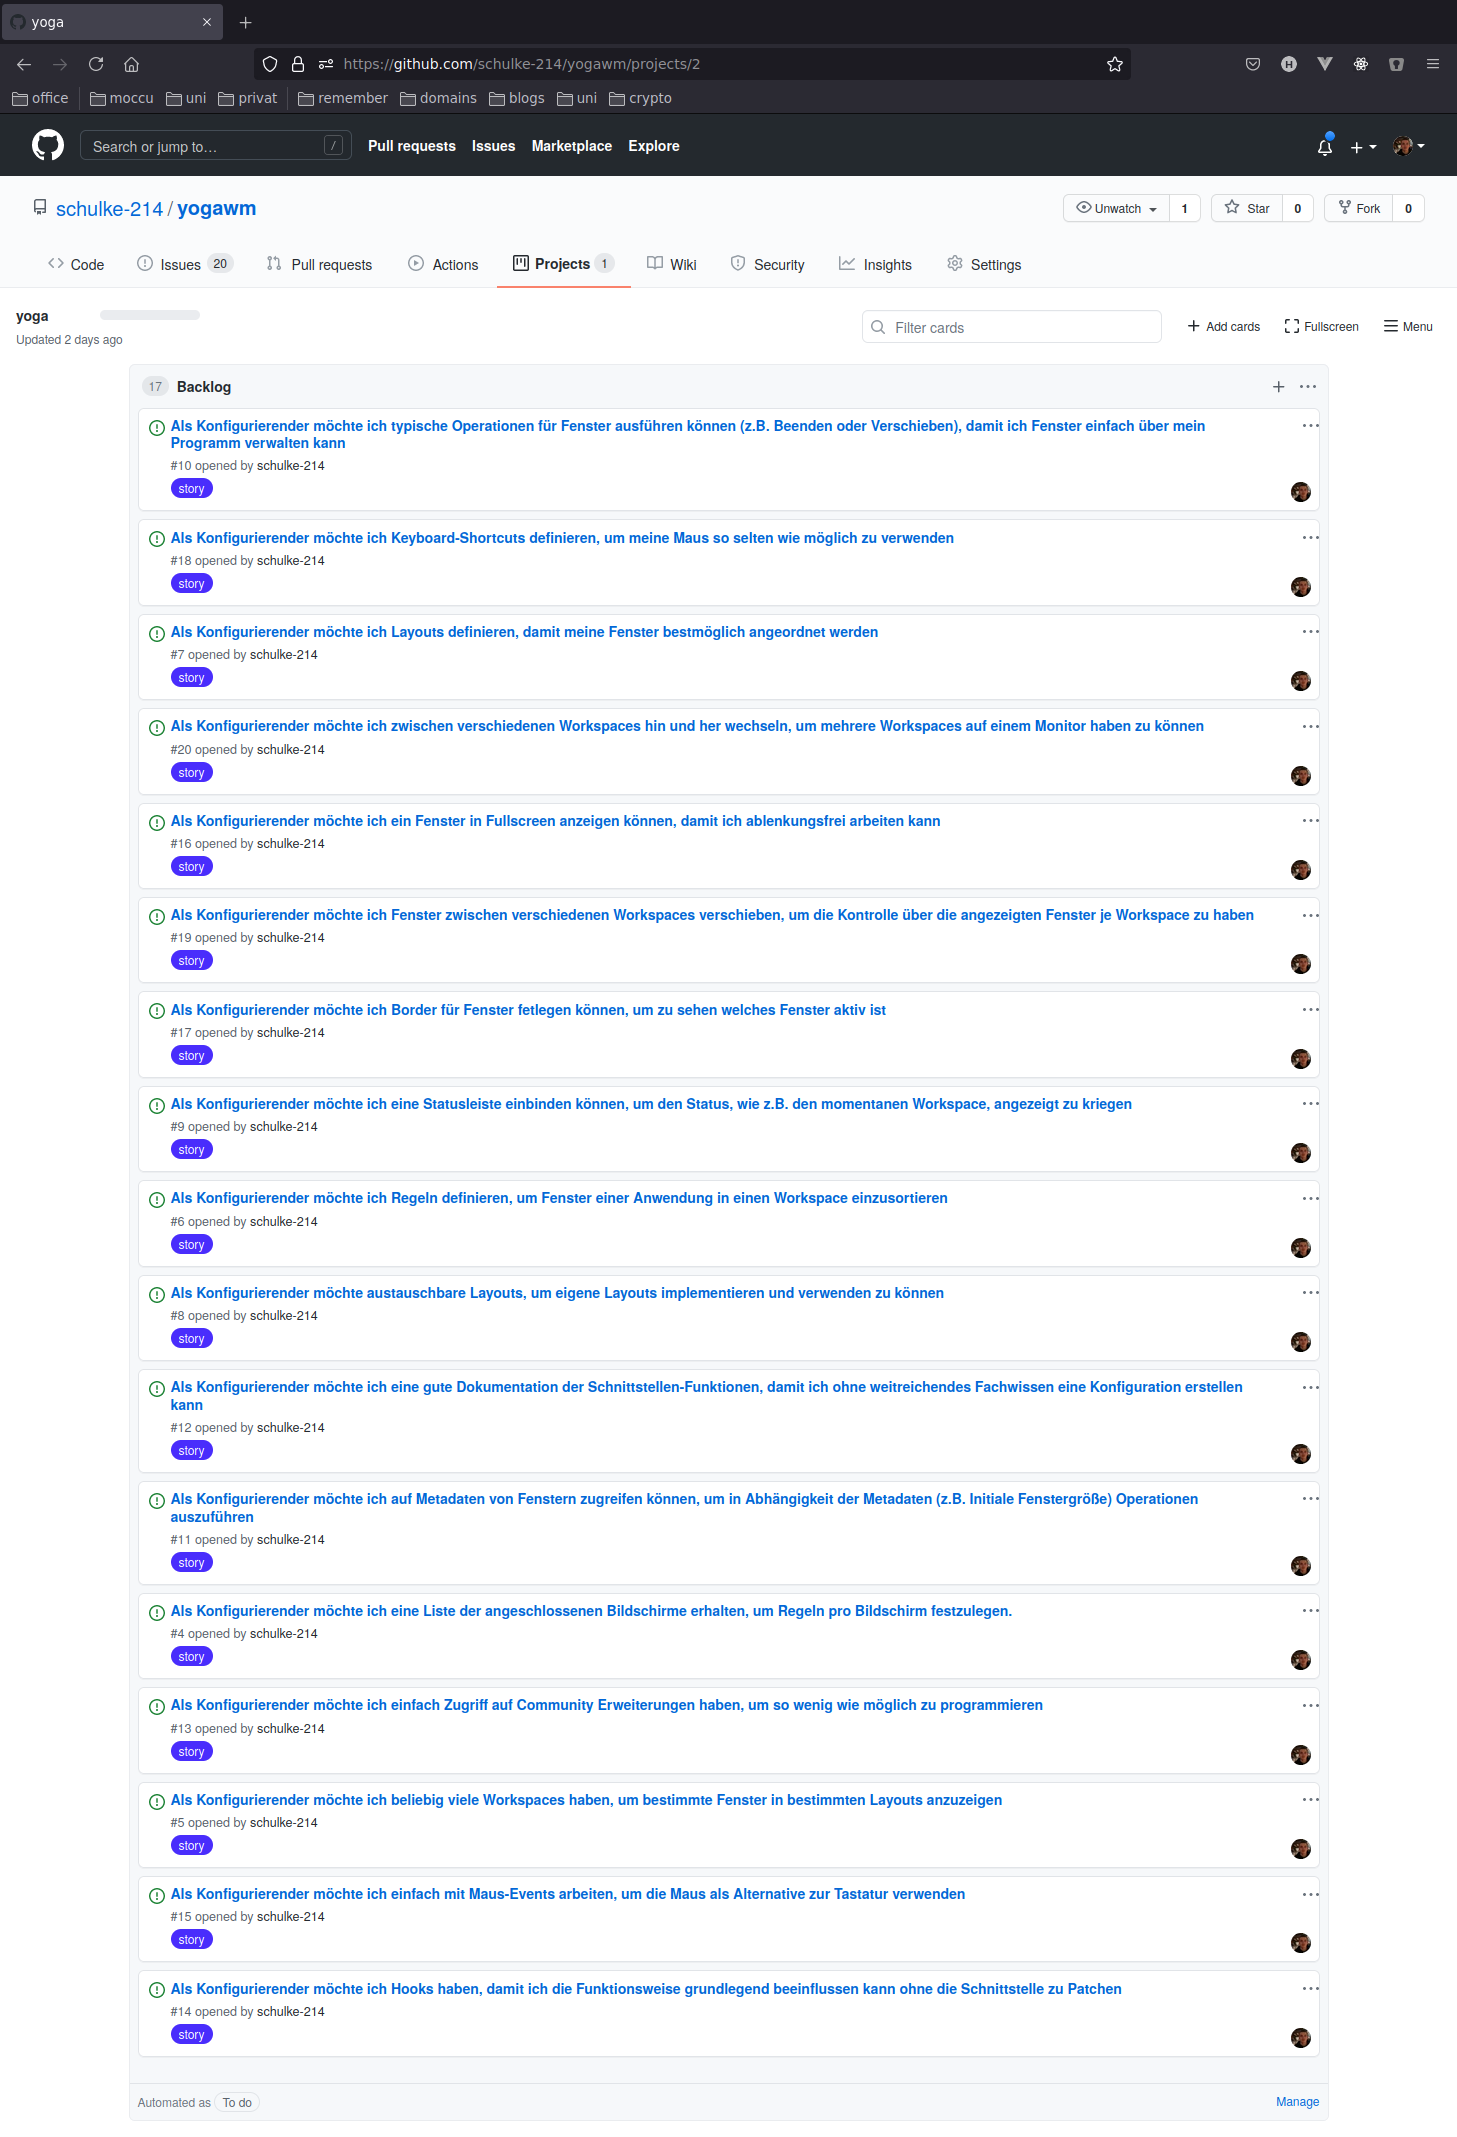
\includegraphics[width=1\textwidth]{product-backlog}
	\centering
	\caption{\emph{Product Backlog}}
	\label{fig:backlog}
\end{figure}

\vspace{1em}

Die Priorisierung der Anforderungen erfolgt relativ über die Reihenfolge im oben gezeigten Product-Backlog.
Innerhalb von GitHub Projects können die einzelnen Stories noch über Flags kategorisiert werden (z.B. als
Funktional oder als Epic)

\subsection{Detaillierte Betrachtung einzelner Anforderungen}

\subsubsection{Details zur User Story \#10}

\begin{tabularx}{\textwidth}{r X}
	\textbf{ID}                 & \#10                                                                                                                                                                            \\
	\\
	\textbf{Story}              & Als Konfigurierender möchte ich typische Operationen für Fenster ausführen können (z.B. Beenden oder Verschieben), damit ich Fenster einfach über mein Programm verwalten kann. \\
	\\
	\textbf{Typ}                & Funktional                                                                                                                                                                      \\
	\\
	\textbf{Akzeptanzkriterien} & Szenario 1 - Fenster schließen
	\begin{quote}
		Gegeben einer gültigen Fenster-Referenz (z.B. durch ID)

		Wenn der Nutzer dieses Fenster schließen will

		Dann schließt sich dieses Fenster
	\end{quote}
	Szenario 2 - Fenster verschieben
	\begin{quote}
		Gegeben einer gültigen Fenster-Referenz (z.B. durch ID)

		Wenn der Nutzer dieses Fenster an eine Stelle (X, Y) bewegen will

		Dann render dieses Fenster auf dem Bildschirm an die Koordinaten
	\end{quote}
\end{tabularx}

\begin{tabularx}{\textwidth}{r X}
	\hspace*{7.75em} & Szenario 3 - Ungültiges Fenster
	\begin{quote}
		Gegeben einer ungültigen Fenster-Referenz (z.B. da das Programm abgestürzt ist)

		Wenn der Nutzer versucht eine Operation (Beenden / Verschieben etc.) auszuführen

		Dann gebe dem Nutzer eine Fehlermeldung zurück
	\end{quote}
\end{tabularx}

\subsubsection{Details zur User Story \#20}

\begin{tabularx}{\textwidth}{r X}
	\textbf{ID}                 & \#20                                                                                                                                             \\
	\\
	\textbf{Story}              & Als Konfigurierender möchte ich zwischen verschiedenen Workspaces hin und her wechseln, um mehrere Workspaces auf einem Monitor haben zu können. \\
	\\
	\textbf{Typ}                & Funktional                                                                                                                                       \\
	\\
	\textbf{Akzeptanzkriterien} & Szenario 1 - Workspace wechseln
	\begin{quote}
		Gegeben einer gültigen Workspace-ID

		Wenn der Nutzer zu dem Workspace wechseln möchte

		Dann verstecke alle Fenster im momentanen Workspace und zeige alle Fenster aus dem Workspace mit der gegebenen ID.
	\end{quote}
	Szenario 2 - Zum letzten Workspace
	\begin{quote}
		Gegeben eines vorherigen Workspace-Wechsels

		Wenn der Nutzer zum letzten Workspace möchte

		Dann verstecke alle Fenster im momentanen Workspace und zeige alle Fenster aus dem vorherigen Workspace.
	\end{quote}
	Szenario 3 - Ungültiger Workspace
	\begin{quote}
		Gegeben einer ungültigen Workspace-ID

		Wenn der Nutzer zu dem Workspace wechseln möchte

		Dann bleibe auf dem momentanen Workspace und gebe dem Nutzer eine Fehlermeldung zurück.
	\end{quote}
\end{tabularx}

\newpage

\subsection{Weitere Merkmale von Anforderungen}

Durch das Issue-Feature von GitHub werden viele Merkmale guter Anforderungen automatisch mit aufgenommen. Zum Beispiel werden
in der Detail-Ansicht eines Issues (die als Story markiert werden kann) immer der Autor, die ID, das Erstellungsdatum, die Historie,
ein Kommentarverlauf / bzw. eine Diskussion zu diesem Issue, der Status (Offen / Duplikat / Closed etc.) und ggf. die Person(en) die gerade
an diesem Issue arbeitet/en festgehalten. \par
Außerdem kann man projektspezifische Templates für Issues anlegen, um z.B. Akzeptanzkriterien / Abnahmeszenarien immer in einem
gewissen Umfang und einer ähnlichen Form zu erfassen.

\begin{figure}[H]
	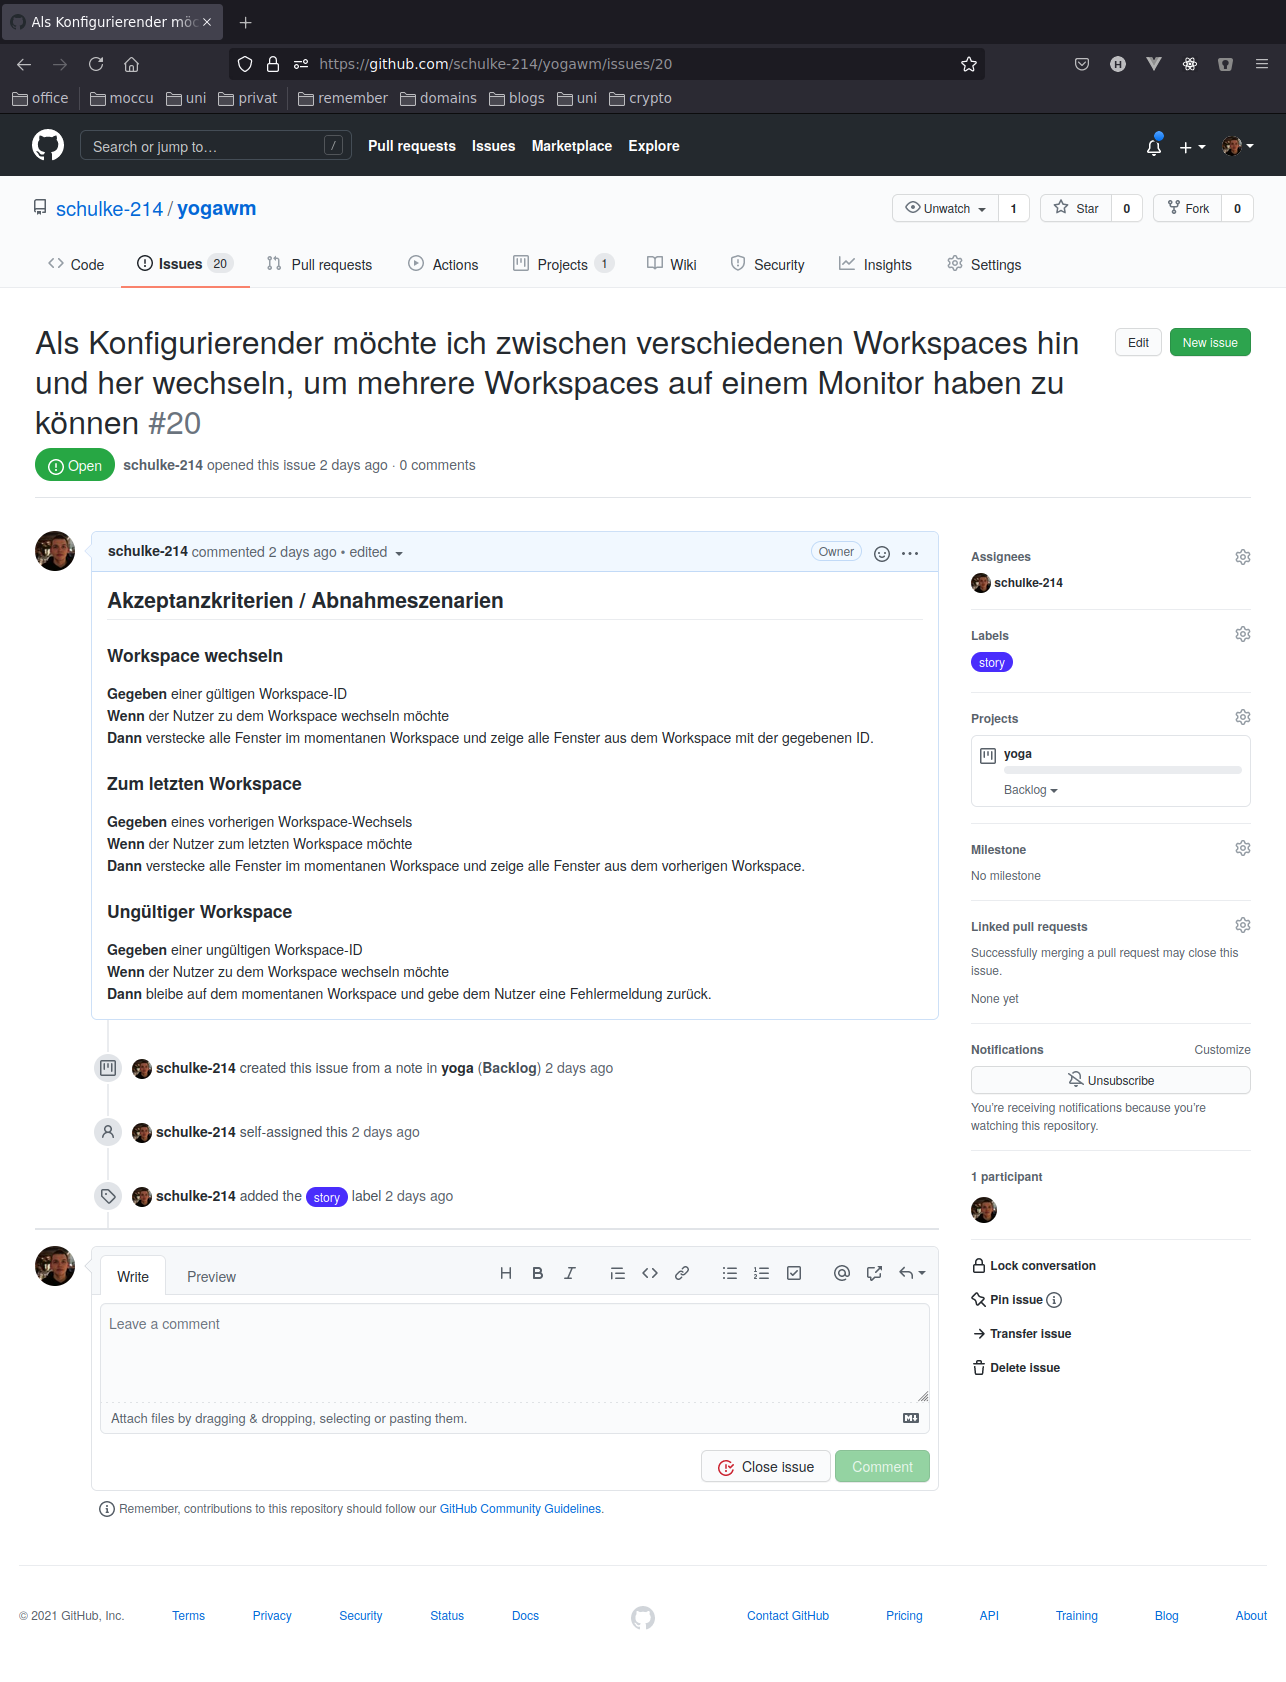
\includegraphics[width=0.8\textwidth]{issue-detail}
	\centering
	\caption{Detail-Ansicht einer Story}
\end{figure}

\end{document}
